\section{Das Model}
Insgesamt werden X(TODO) verschiedene Konfigurationen getestet. Sie unterscheiden sich in der Baumgröße, Waldgröße, Featureauswahl, Ensemble-Methode, sowie in Blattgröße und Quantifizierungsschwellenwert.
\newline
\begin{figure}
    \centering
    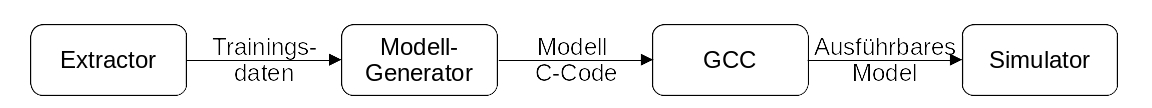
\includegraphics[width=\linewidth]{images/model_workflow.jpg}
    \caption{Arbeitsablauf um ein Model zu trainieren und zu validieren.}
    \label{fig:model_workflow}
\end{figure}
\newline
Jeder Entscheidungswald wird mit dem Python-Modul \texttt{Scikit-Learn} trainiert. Scikit-Learn implementiert den Konstruktionsalgorithmus CART (siehe Sektion \ref{sec:construction}) für den Entscheidungsbaum und bietet
zusätzlich zahlreiche Ensemble-Methoden an. Jede Konfiguration folgt den in Abbildung \ref{fig:model_workflow} illustrierten Arbeitsablauf.
\newline
\newline
Zunächst wird die Trainingsmenge vorverarbeitet. Dabei werden die verschiedenen
Features extrahiert, die während der Konstruktion eines Entscheidungsbaumes benötigt werden. Dann wird das Model mit Scikit-Learn und den gegebenen Konfigurationsparametern generiert. Anschließend wird aus dem Model
ausführbarer C-Code generiert und kompeliert. Zuletzt wird die Erkennungsgenauigkeit des ausführbaren Models auf der Testmenge von Klisch und Dymel ermittelt.

\subsection{Training}
\label{sec:Training}
Mit Scikit-Learn werden Wahl basierte Entscheidungswaldklassifizierer mit den in Sektion \ref{sec:Ensemble} genannten Ensemble-Methoden trainiert. Insgesamt werden Waldgrößen zwischen 1 bis 16 betrachtet und
Maximalhöhen von den einzelnen Entscheidungsbäumen zwischen 1 bis 22. Außerdem werden die Blattgrößen, d. h. die minimale Anzahl von Trainingsdateneinträgen pro Blatt, \textit{1, 2, 4 und 8} sowie die
Quantifizierungsschwellenwerte, d. h. Zuwachs der Entscheidungsgenauigkeit pro Teilbaum, \textit{0, $10^{-3}$, $10^{-2}$ und $10^{-1}$} betrachtet.
\newline
\newline
Die letzten beiden Parameter verringern potentiell die Erkenneungsgenauigkeit von den einzelnen Entscheidungsbäumen, sie verringern aber auch die Größe des Baumes signifikant.
Dadurch können bessere Entscheidungswälder gefunden werden, die zuvor nicht in den Programmspeicher eines Arduino Boards gepasst haben (siehe Sektion \ref{sec:eval_size}).
\newline
\newline
Die Konstruktion der Entscheidungswälder ist nicht deterministisch. Zuallererst muss die Konstruktion eines einzelnen Entscheidungsbaumes nicht deterministisch sein, da selbst wenn immer die beste Teilung
ausgewählt wird, können mehrere Teilungen auch gleich gut sein. Aus diesen müsste zufällig eine ausgewählt werden. Folglich ist jede Ensemble-Methode zufällig. Außerdem wählt die RandomForest-Methode
zufällig eine Featureauswahl, und die Bagging-Methode partitioniert die Trainingmenge zufällig. Aus diesem Grund kann in Scikit-Learn einen \texttt{random\_state} zuweisen, der den \textit{Seed} des
unterliegenen Zufallszahlengenerators setzt.
\newline
\newline
Dementsprechend kann man die Konstruktion als Monte Carlo Algorithmus betrachten, d. h. wiederholte Ausführungen erhöhen die Wahrscheinlichkeit, dass das beste Ergebnis dieser Konfiguration gefunden wurde.
Jede Konfiguration wird aus diesem Grund mit 140 verschiedenen \texttt{random\_state} ausgeführt.
\newline
\newline
Zum trainieren wird eine Kombination aus der Trainingsmenge von Fey und Kubik verwendet, sowie 25\% der Gestenmenge und 12,5\% der Nullgestenmenge von Dymel (siehe Sektion \ref{sec:DymelData}). Insgesamt 7629
Ausführungen der Handgesten. Davon werden 50\% zufällig zum trainieren genutzt und die überbleibenden 50\% werden genutzt, um den besten Entscheidungswald aus den 140 verschiedenen \texttt{random\_state}
zu ermitteln.

\subsection{C-Code Generierung eines Entscheidungsbaumes}
\label{sec:cCodeTree}
Das Model soll auf kleinen eingebetteten Systemen ausgeführt werden. Diese haben eine Toolchain um die Firmware zu generieren, die meistens auf der Programmiersprache \texttt{C} basiert. Dies trifft auch auf das in
dieser Arbeit benutzten Arduino Board zu.
\begin{lstlisting}[label=lst:sklearnTreeStructure,caption={Skizze der rekursiven Datenstruktur für Entscheidungsbäume die von Scikit-Learn genutzt wird.}]
enum Knoten<T> {
    Blatt(Vec<usize>),
    Elternknoten {
        test: (features: Vec<T>) -> bool,
        knoten_links: Knoten<T>,
        knoten_rechts: Knoten<T>
    }
}
\end{lstlisting}
Das Model wird mit dem Python-Modul Scikit-Learn generiert. Dementsprechend muss aus der internen Repräsentierung von Scikit-Learn das Model extrahiert werden. Scikit-Learn definiert eine rekursive Datenstruktur in
der jedes Blatt für jede Klassifizierungsklasse die Anzahl der Trainingsdateneinträge enthält, die nach dem traversieren aller Test in diesem Blatt eingeordnet werden. Jeder Elternknoten besteht aus einem Test der
ein Feature mit einem Schwellenwert vergleicht und einen Knoten für jedes Ergebniss dieses Tests (siehe Listing \ref{lst:sklearnTreeStructure}). Im Falle von Scikit-Learn ist der der Test immer
ein $\leq$ Vergleich, weswegen es genau zwei Kindknoten gibt.
\begin{lstlisting}[label=lst:sklearnCCodeParent,caption={C-Code eines Elternknotens.}]
if (features[k] <= X) {
    Traversiere Kind Links...
} else {
    Traversiere Kind Rechts...
}
\end{lstlisting}
Ein Elternknoten wird dementsprechend als ein \texttt{if (test) \{ \ldots\ \} else \{ \ldots\ \}} Ausdruck modeliert (siehe Listing \ref{lst:sklearnCCodeParent}). Dabei ist der \texttt{test} ein $\leq$ Vergleich eines
Features mit einem Schwellenwert und der Inhalt der einzelnen Blöcke ist abhängig von den Kindesknoten.
\begin{lstlisting}[label=lst:sklearnCCodeLeaf,caption={C-Code eines Blattes.}]
result[0] = (Anzahl Klasse 1) / (Gesamtanzahl im Blatt);
...
result[N] = (Anzahl Klasse N) / (Gesamtanzahl im Blatt);
return;
\end{lstlisting}
Der C-Code im Blatt ist abhängig von dem Wahlklassifizierer. Man kann entweder die Klasse auswählen, die von den meisten Bäumen klassifiziert wurde, oder die
Erkennungswahrscheinlichkeiten jedes Baumes im Ensamble wird summiert und davon wird die Klasse mit der größten Summe ausgewählt (siehe Sektion \ref{sec:wahlklassifizierer}).
In dieser Arbeit wurde sich für letzteres entschieden. Im C-Code wird das modeliert durch die Zuweisung der Wahrscheinlichkeiten der einzelnen Klassen im Blatt zu dem Ergebnisparameter
\texttt{result} (siehe Listing \ref{lst:sklearnCCodeLeaf}).

\subsection{C-Code Generierung eines Entscheidungswaldes}
Ein Entscheidungswald besteht aus einem Ensamble von Entscheidungsbäumen. Bei der Evaluierung eines Entscheidungswaldes wird der jeder Entscheidungsbaum evaluiert und die Ergebnisse zusammengefasst, z. B.
durch einen Wahlklassifizierer.
\begin{lstlisting}[label=lst:sklearnCCodeTreeFunction,caption={C-Code Funktionskopf eines Baumes $i$.}]
function tree_i(float* features, float* result);
\end{lstlisting}
Zunächst wird jeder Entscheidungsbaum als Funktion isoliert (siehe Listing \ref{lst:sklearnCCodeTreeFunction}). Als Eingabeparameter dienen die extrahierten Features und ein Float-Array \texttt{result}, dass das
Ergebnis speichert.
\begin{lstlisting}[label=lst:sklearnCCodeTreeVoting,caption={C-Code des Wahlklassifizierers mit $N$ Klassen und $K$ Bäumen.}]
float tree_res[N] = { 0.0, ..., 0.0 };
float total_res[N] = { 0.0, ..., 0.0 };
unsigned char result_map[N] = { ... };

// Wiederhole dies für K Bäume
tree_i(features, tree_res);
total_res[0] += tree_res[0];
...
total_res[N-1] += tree_res[N-1];

unsigned char max_index = 0;
float max_value = 0;
for (unsigned char i = 0; i < N; ++i) {
    if (max_value < total_res[i]) {
        max_value = total_res[i];
        max_index = i;
    }
}
return result_map[max_index];
\end{lstlisting}
Listing \ref{lst:sklearnCCodeTreeVoting} zeigt wie ein Ensamble bestehend aus $K$ Entscheidungsbäumen, die jeweils $N$ mögliche Klassifizierungsergebnisse zurückgeben, mit der Wahlklassifizierungsmethode
evaluiert wird. Zunächst wird jeder Baum evaluiert und die Ergebnisse summiert. Anschließend wird die Klasse mit dem maximalen Wert zurückgegeben.